
\setcounter{chapter}{1}
\chapter{Requirement Specification and Overall Architecture}
\minitoc %insert la minitoc
\graphicspath{{Chapitre2/figures/}}

%\DoPToC

%==============================================================================
\pagestyle{fancy}
\fancyhf{}
\fancyhead[R]{\bfseries\rightmark}
\fancyfoot[R]{\thepage}
\renewcommand{\headrulewidth}{0.5pt}
\renewcommand{\footrulewidth}{0pt}
\renewcommand{\chaptermark}[1]{\markboth{\MakeUppercase{\chaptername~\thechapter. #1 }}{}}
\renewcommand{\sectionmark}[1]{\markright{\thechapter.\thesection~ #1}}

\begin{spacing}{1.2}
    %==============================================================================
    \section*{Introduction}
    The requirement specification is the first step in the software development process.
    It is the basis for the design and implementation of the software system.
    It is the process of defining, documenting and maintaining the requirements of the system.
    The requirements are the description of the system services and constraints that are to be implemented.

    In this chapter we will present the requirement specification of the project, we will define our actors,
    the functional and non-functional requirements of the system.
    We will also present the overall architecture of the project and the design principles that we will follow.

    \section{Requirement Specification}

    \subsection{Actors Identification}
    Our library is developed for one main actor: the scientist.\\
    The scientist is the person who is going to use the library to develop new data processing algorithms,
    acquire data from different IO sources, analyze the data and visualize the results.
    It is assumed that the scientist is very competent but is not necessarily an expert in software development.
    The library is designed to be easy to use and to provide a high level of abstraction to the scientist.



    \subsection{Functional Specification}
    \subsubsection{File Input/Output}
    The library should provide the scientists an interface to handle file input/output:
    \begin{itemize}
        \item Read/Write frame data from different file formats: Raw, JSON, HDF5 and Numpy.
        \item Reorder the binary frame data according to the detector type.
        \item In case of part files (data split accross multiple files), the library should be able to read all the files and reconstruct the data.
        \item Read/Write metadata from different file formats: JSON, Raw.
        \item Define a new cluster file format (.clust2) to store cluster data. The file format must
              be flexible to accomodate different types of structured data.
        \item Read/Write from the new cluster file format.
    \end{itemize}

    \subsubsection{Network Input/Output}
    The library should provide the scientists an interface to handle network input/output:
    \begin{itemize}
        \item Read frame data from multiple receivers using ZeroMQ. \cite{hintjens2013zeromq}
        \item Synchronize the data streams coming from different receivers and merge them into a single data stream.
        \item Send data to multiple server using ZeroMQ. Thses servers can be other existing GUI applications.
        \item Provide an interface to distribute tasks accross multiple workers using ZeroMQ.
    \end{itemize}

    \subsubsection{Data Processing}
    Although the task of data processing is very specific to the scientist, the library should provide a set of
    basic data processing algorithms that can be used as building blocks for more complex algorithms.
    In addition implementing these basic algorithms will help the scientist to understand the library and how to use it.
    Therefore helps in acclerating the adoption of the library.

    Specifically the library should implement a cluster finder algorithm that can be used to find clusters in a frame of data.
    and also a pedestal subtraction algorithm that can be used to remove the background noise from the data.

    \subsubsection{Python Interface}

    Most scientists prefer to use Python for their data analysis tasks. Python has
    become the de facto language for data analysis and machine learning.
    It is easier to use than C/C++ and is less verbose. It has a large number of libraries
    that can be used for data analysis and visualizations.

    Therefore the library should provide a Python interface that can be used to access its functionalities.
    The Python interface should be easy to use, similar to other Python libraries like Numpy and Pandas.


    \subsection{Non-Functional Specification}
    \subsubsection{Performance}
    The library is expected to handle around 10GB/s of data streaming from the network and process it in real time.
    In addition processing large data files should be done as fast as possible to allow the scientist to iterate quickly on their work.
    These are very challenging requirements and will require a lot of optimization in all levels of the library.
    The library should be able to run on a single CPU core and also on multiple CPU cores to parallelize the processing.

    \subsubsection{Reliability}
    The library should be able to handle different types of errors that can occur during the data processing.
    It should be able to recover from these errors and continue processing the data.
    The library should also be able to handle different types of data corruptions that can occur during the data acquisition.
    For example in case of a network error, the software should reconnect to the network and continue receiving the data.
    Furthermore, Thorough testing on multiple levels and on different scenarios is required to ensure the integrity of the code.

    \subsubsection{Portability}
    Nothing is assumed about the platform on which the library will run. It must be able to run on different operating systems (Windows, Linux, MacOS).
    and on different hardware architectures (x86, ARM). It cannot rely on specific kernel features or syscalls that are not available on all platforms.


    \subsubsection{Extensibility}
    Use cases and requirements can change over time. The library should be able to adapt to these changes.
    The software design must allow developers and scientists to add new functionalities easily.
    Careful considerations must be taken to make easy to add features without breaking the existing code.


    \subsubsection{Maintainability}
    The development of the library is expected to continue for a long time. The library should be easy to maintain and evolve.
    The code should be well documented and easy to read. Explanations should be provided for complex algorithms and data structures.
    Helpful documents should be provided to help new developers understand the code and how to contribute to the project.

    \subsection{Requirements Specification Analysis}
    First, given the harsh performance requirements, the library should be implemented in a compiled language.
    Rust, C++, Java are possible candidates for this task. Rust is a new language that is gaining popularity for systems programming.
    It is designed to be safe and fast \cite{bugden2022rust}. However, it is still a young language and the ecosystem is not as mature as C++.
    Java is a good candidate for performance and portability, but it is not as fast as C++.
    Therefore, C++ is the best candidate for this task. It is a mature language with a large ecosystem and a large number of libraries that can be used.
    It is also a very fast language that can be optimized to run close to the hardware. Plus, it is used in many related scientific solutions.\\

    Second, to provide high performance python code, the library should be implemented in C++ and then wrapped in Python using the Pybind11 library \cite{pybind11}.
    Pybind11 is a lightweight header-only library that exposes C++ types in Python and vice versa, mainly to create Python bindings of existing C++ code.
    It is easy to use and provides a high level of abstraction to the developer. It is also very fast and does not introduce a lot of overhead.\\
    

    Third, it is possible to modularize the library into different modules where each module is responsible for a specific domain.
    This will help in organizing the code and make it easier to maintain and evolve. It will also help in parallelizing the development of the library.
    The library can be divided into the following modules:
    \begin{itemize}
        \item core module: responsible for the basic data structures that will be used in all other modules.
        \item file\_io module: responsible for reading and writing data from different file formats.
        \item network\_io module: responsible for reading and writing data from the network.
        \item processing module: responsible for implementing the data processing algorithms.
        \item python module: responsible for exposing the library to Python.
    \end{itemize}

    Fourth, for more flexibility and extensibility, the library should be implemented using the Clean Architecture and the SOLID principles.

    Finally, extensive testing is required to ensure the reliability of the library. Unit tests, integration tests and end to end tests are all required.
    In addition to that, the library should be tested on different platforms and different hardware architectures to ensure its portability.















    \section{Overall Architecture and Guidelines}
    Given the requirements of the project, software architecture and design principles must be carefully chosen to ensure the success of the project.
    In this section we will present some of the design principles and architectural patterns that we will follow in the project.
    \\

    A software solution should provide to stakeholders two main things: behavior and structure.
    The behavior is the functionality of the system, what the system does. It answers for the functional and non-functional requirements of the system.
    The structure is the organization of the system, how the components of the system are organized and how they interact with each other.
    A good structure is essential for the maintainability and extensibility of the system.
    \\

    Investing time in the design of the software architecture is very important. Specifications can change, requirements can change, but the architecture is the foundation of the system and
    it should be solid and flexible enough to accommodate these changes.
    \begin{quote}
        The goal of software architecture is to minimize the human resources required to build and maintain the required system
        \begin{flushright}
            Robert C. Martin \cite{clean}
        \end{flushright}

    \end{quote}

    As the quote by "Uncle Bob" suggests, the goal of software architecture is to reduce the software development costs in the project's early life. But also it is
    crucial to bring down the cost of new features and maintenance as project evolves and becomes more complex.
    \\

    Several architectural patterns exist such as: Layered Architecture, Hexagonal Architecture \cite{freeman2009growing}, Clean Architecture \cite{clean}, Onion Architecture \cite{Onion}, DCI \cite{dci} etc.
    Although these patterns differ they share some common principles such as separation of concerns, testability, and independence from frameworks, databases, and UIs.
    \\

    In this project we will follow the Clean Architecture.


    \subsection{Clean Architecture}
    The clean architecture was first introduced by Robert C. Martin (also known as Uncle Bob)
    in his blog post \cite{cleanBlog} and later in his book "Clean Architecture: A Craftsman's Guide to Software Structure and
    Design" \cite{clean}. Like other architectural patterns, the clean architecture promotes
    separation of concerns, testability, and independence from frameworks, databases, and UIs.

    As shown in figure \ref{fig:clean}, the clean architecture is composed of several layers:
    \begin{itemize}
        \item Entities: This layer contains the business objects of the system. These objects are the core of the system and they are independent of any other layer.
        \item Use Cases: This layer contains the application-specific business rules. It contains the use cases of the system. Each use case is a single action that the system can perform.
        \item Interface Adapters: This layer contains the interfaces that the system uses to communicate with the outside world. It contains the presenters, controllers, and gateways.
        \item Frameworks and Drivers: This layer contains the frameworks and drivers that the system uses. It contains the web frameworks, databases, and other external systems.

    \end{itemize}

    \begin{figure}
        \centering
        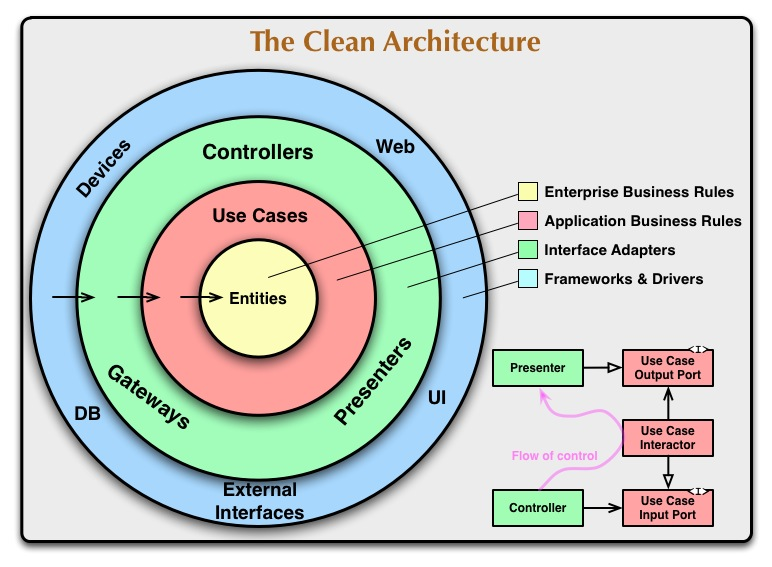
\includegraphics[scale=0.5]{Chapitre2/figures/CleanArchitecture.jpg}
        \caption{Diagram of the Clean Architecture: the circles represent the different
            layers of the architecture, the arrows represent the dependencies between the layers.
            The bottom right part of the diagram shows how dependencies are inverted.}
        \label{fig:clean}
    \end{figure}

    The clean architecture promotes the separation of concerns and the independence of the layers. Each layer is independent of the other layers and can be replaced without affecting the other layers.
    It is very important that the inner circles do not depend on the outer circles. The inner circles
    will not know anything about functions, classes, or modules in the outer circles. This known as
    the \textbf{Dependency Rule}.
    \begin{quote}
        "This rule says that source code dependencies can only point inwards. Nothing in an inner circle can know anything at all about something in an outer
        circle." \cite{cleanBlog}

    \end{quote}

    For communication between the layers, interfaces are used. The inner layers define interfaces that
    the outer layers must implement or call. The dependency inversion principle (will be explained in the next section) is used
    to decouple the layers and make them independent of each other.


    \subsection{SOLID Principles}
    The SOLID principles are a set of five principles that are used to design object-oriented software.
    They were introduced by Robert C. Martin in his paper "Design Principles and Design Patterns" \cite{martin2000design}.
    \subsubsection{Single Responsibility Principle (SRP)}
    The SRP states that:
    \begin{quote}
        "A module should have only one reason to change." \cite{clean}
    \end{quote}

    This means that a class should have only one responsibility and serves one actor. If a class
    has more than one responsibility, it should be split into multiple classes. This will make the
    code easier to understand and maintain.

    \subsubsection{Open/Closed Principle (OCP)}
    The OCP states that:
    \begin{quote}
        "A software artifact should be open for extension but closed for modification." \cite{meyer}
    \end{quote}

    This means that the code should be designed in such a way that its features can be extended
    without the need to modify the existing code. This can be acheived by a plethora of design patterns and
    object oriented principles.

    \subsubsection{Liskov Substitution Principle (LSP)}
    As Barbara Liskov defined it in 1988:
    \begin{quote}
        "If for each object o1 of type S there is an object o2 of type T such that for
        all programs P defined in terms of T, the behavior of P is unchanged when o1 is
        substituted for o2 then S is a subtype of T" \cite{liskov}
    \end{quote}

    Or in simpler terms: Subtypes must be substitutable for their base types. In the case of classes
    this means that a subclass should be able to replace its parent class without affecting the
    correctness or behavior of the program.

    \subsubsection{Interface Segregation Principle (ISP)}
    The ISP states that:
    \begin{quote}
        "Clients should not be forced to depend on methods that they do not use." \cite{agileMartin}
    \end{quote}

    This means that interfaces should be small and focused.  The ISP combats the problem of interface pollution. When classes
    depend on an interface it does not fully use, it is forced to implement or depend on methods
    that are not needed. This can lead to unnecessary dependencies and coupling between classes.
    and code might break when the interface is updated.

    The solution proposed by the ISP is to split the interfaces into smaller interfaces that are
    more focused. This way the classes can depend on the interfaces that they need and not on the
    "fat" interface.

    \subsubsection{Dependency Inversion Principle (DIP)}
    The DIP is defined in the Agile Software Development book by Robert C. Martin \cite{agileMartin} as:
    \begin{quote}
        \begin{itemize}
            \item High-level modules should not depend on low-level modules. Both should depend on abstractions.
            \item Abstractions should not depend on details. Details should depend on abstractions.
        \end{itemize}
    \end{quote}

    The dependency inversion principle is crucial for the successful implementation of the clean architecture.
    It is used to decouple the layers and make them independent of each other. The DIP is the mechanism
    that allows the inner layers to define interfaces that the outer layers must implement or call.
    This way the inner layers do not depend on the outer layers and can be replaced without affecting the other layers.

    \subsection{C++ Specific Design}
    The library will be implemented in C++ and will be wrapped in Python. For this reason
    some specific design considerations must be taken into account. C++ is a very powerful
    language that provides a lot of features that can be used to implement almost any design.
    However, it is also a very complex language that has its own pitfalls and limitations.

    \subsubsection{Templates Metaprogramming}
    C++ provides a powerful feature called templates that can be used to implement metaprogramming.
    Metaprogramming is the writing of programs that write or manipulate other programs.
    Templates allows the programmer to write generic code that will be instantiated at compile time.
    This can be used to implement generic algorithms that can work with different types of data.
    Templates can make the code much more efficient as it moves the computation from runtime
    to compile time. \\

    Templates are a core design feature of C++. They are used extensively in the C++ standard
    library and in many other libraries. However, templates can be very complex and can lead to
    very long compile times and cryptic compile error messages.\\

    From a software design perspective, being aware of templates and how to use them is very
    important. Templates can be used for static polymorphism, to implement generic algorithms,
    and to implement compile-time checks.\\

    The very important constraint to keep in mind for this project is that the C++ library will
    be wrapped in Python. In practice this is done by shared libraries that are loaded by the Python
    interpreter. Hence, the C++ code must be compiled first before it can be used in Python.

    \begin{lstlisting}[language=C++,caption={Example of a Templated Function},label={lst:label}]
template <typename T, int n>
T add(T a) {
    return a+n;
}
    \end{lstlisting}

    In the above example \ref{lst:label}, the function add is a templated function that takes
    a type T and an integer n as template parameters. The function adds n to the input parameter
    a and returns the result.\\

    In C++ code whenever we call this function with a different set of parameters
    the compiler will generate a new version of the function. However, in Python we cannot do
    this as the interpreter will not be able to generate new versions of the function at runtime.\\

    Therefore, the use of templates in the C++ code must be limited to the minimum and only used
    when it is really necessary. The C++ code should be as generic as possible but not at the
    expense of the Python interface.\\

    In some use cases we are able to instantiate the C++ templated code for a set of types or values
    that the function expects. For example we can define function for numerical types (int8, int16, uint8, uint16, float, double ...)
    However we should always be aware that this can lead to code bloat and increase the size
    of the shared library.\\





    \subsubsection{C++ Idioms}
    C++ is an "old" language that has evolved over the years. It offers a lot of complex
    features that can be combined to create very powerful and efficient code. It also has limitations
    especially as it is not memory safe and it is easy to introduce bugs.\\

    For this reason, it is important to follow some idioms and best practices when writing C++ code.
    Some of the most important idioms are:\\ \\
    \textbf{RAII (Resource Acquisition Is Initialization)}:
    This idiom states that important resources' lifecycle should be bound to the lifetime of
    an object. This way the resource is automatically acquired when the object is constructed and
    released when the object goes out of scope. Another name for this idiom is
    Scope Bound Resource Management.\\

    One of the most common errors in C++ is allocating memory, opening files or sockets and forgetting
    to release them. This can lead to leaks in the program and can cause the program to crash.
    The RAII idiom is widely used to avoid these problems.\\

    As this project will use a lot file pointers, sockets and memory resources, it is very important
    to wrap these resources in RAII objects. This will ensure that the resources are released when
    they are no longer needed.\\


    \textbf{Curiously Recurring Template Pattern (CRTP)}:
    The CRTP is a design pattern that is used to add functionality to a class by inheriting
    from a base class. The base class is a template class that takes the derived class as a
    template parameter. This allows the base class to access the members of the derived class.\\

    \begin{lstlisting}[language=C++,caption={Example of CRTP},label={lst:crtp}]
template <typename T>
class Base {
    void foo() {
        static_cast<T*>(this)->bar();
    }
};

class Derived : public Base<Derived> {
    void bar() {
        // do something
    }
};        
    \end{lstlisting}

    In the above example \ref{lst:crtp}, the class Base is a template class that takes a type T
    as a template parameter. The class has a function foo that calls the function bar of the
    derived class. The derived class must inherit from the base class and pass itself as the
    template parameter.\\

    It is a technique that involves using inheritance and static polymorphism to achieve a
    form of compile-time polymorphism. Indeed the CRTP allows for compile-time optimization
    and inlining of code since the method calls are resolved at compile time. It also
    eliminates the runtime overhead associated with virtual function calls, making it
    suitable for performance-critical code.\\


    \textbf{Type Erasure}
    Type erasure is a programming technique in C++ used to enable polymorphism without
    sacrificing performance or introducing unnecessary runtime overhead. It allows the
    creation of interfaces and containers that can work with objects of different types
    in a type-safe manner while deferring the determination of the actual types until runtime.\\

    Type erasure is often used to implement generic programming in C++ where the type of
    the objects is not known at compile time. It is also used to implement interfaces that
    can work with objects of different types.\\

    the std::function and std::any classes in the C++ standard library are examples of type
    erasure. They allow the creation of objects that can hold objects of different types
    and call their methods without knowing the actual type of the object.\\

    \begin{lstlisting}[language=C++,caption={Example of Type Erasure},label={lst:erasure}]
Shape circle = Circle(5);
Shape square = Square(5);
std::vector<Shape> shapes;
    \end{lstlisting}

    In the above example \ref{lst:erasure}, the Shape class is a base class that is used to
    store objects of different types. The Circle and Square classes are derived from the Shape
    class. The vector shapes is a vector of Shape objects that can hold objects of different types.\\

    \textbf{Pimpl (Pointer to Implementation)}:
    The Pimpl idiom is used to hide the implementation details of a class from the user of the
    class. It is used to reduce the compile time dependencies and to hide the implementation
    details of the class.\\ \\

    The list of the mentioned idioms is not exhaustive. C++ offers a lot more idioms and best 
    practices that can be used to write efficient and safe code.








    % \subsubsection{C++ Limitations}
    % C++ is a very powerful and influential language that has been used to implement some of the
    % most complex and efficient software systems. However, it is also a very complex language

    % TODO: describe the limitations of C++
    % \begin{itemize}
    %     \item Memory Management: no gc
    %     \item Error Handling:
    %     \item Compilation Time:
    %     \item Complexity:
    %     \item strong typing
    %     \item inheritance only with pointers or references

    % \end{itemize}

    \subsection{Project Architectural Design}
    Having armed ourselves with various design principles and architectural patterns, we can now
    tackle the task of designing the architecture of the project.
    \subsubsection{Project Modules}
    Having identified the different requirements of the project, we can now divide the project into
    different modules. Each module will be responsible for a specific domain of the project.

    \begin{itemize}
        \item file\_io module: Responsible for handling file input/output operations.
        \item network\_io module: Responsible for handling network operations.
        \item processing module: Responsible for implementing the data processing algorithms.
        \item core module: Responsible for the basic data structures that will be shared between other modules.
        \item python module: Responsible for exposing the library to Python.
    \end{itemize}

    Each module should be independent of other modules and communicates with them through exposed interfaces.
    Furthermore, each module includes its own tests. This will help in isolating the tests
    and make it easier to test the modules. In general this approach focuses on separation of
    concerns and modularity.\\

    \subsubsection{Project Architecture}

    \begin{figure}
        \centering
        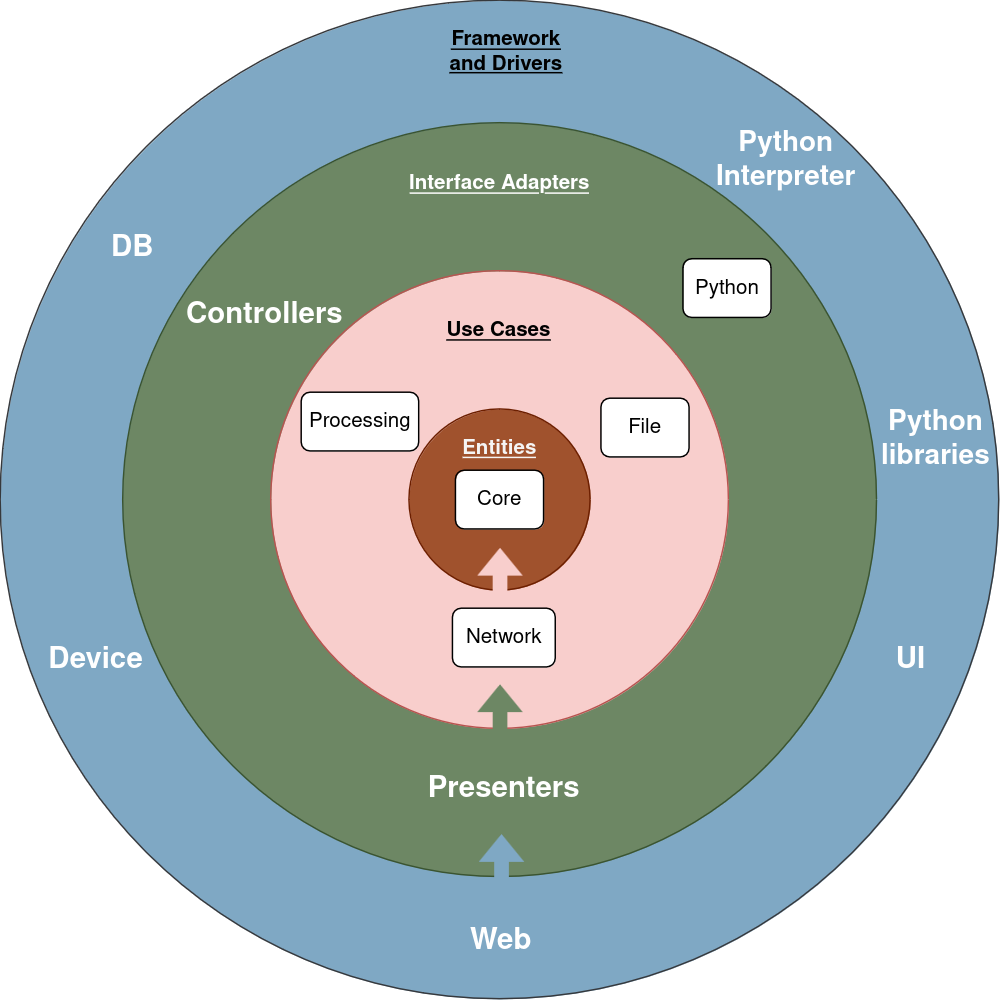
\includegraphics[width=\textwidth]{Chapitre2/figures/aare.png}
        \caption{Diagram of the Project Architecture}
        \label{fig:arch}

    \end{figure}

    The project will follow the Clean Architecture. The project will be divided into different
    layers where the inner layers do not depend on the outer layers. \\

    Figure \ref{fig:arch} is an illustration of how the project is organized.
    Boxes represent the modules that have been implemented by the project. Controllers and
    Presenters are not implemented but in future iterations they can be added to communicate with a UI or
    an API. The direction of the arrows represents the dependencies between the modules.\\

    The core module is at the center of the architecture.
    It is the most stable part of the software and least likely to change. core module will
    contain data structure such as "\lstinline|Frame|" and "\lstinline|Cluster|" that will be used by higher level modules.
    The core module will also contain the interfaces that will be used by the other modules.\\

    One level above the core module we find the file\_io, network\_io and processing modules.
    These modules contain the application-specific business rules and use cases.
    These modules will also depend on the core module.\\

    In the Interfaces and Adapters layer we can find the python module. This module will be written in C++
    and it will contain the bindings to expose the libraries functionalities. The python module
    will depend on all the modules below it. In case of future changes, this layer can contain
    Presenters to present the data on a GUI or in another formats and also it can contain
    controllers to handle requests from other servers or the Web.\\

    Finally, the Frameworks and Drivers layer will contain the external components that the system
    will use. Hardware, Databases, Python libraries etc all reside in this layer. These components
    are subject to frequent unpredictable changes and should be isolated from the rest of the
    system.\\


    % \subsubsection{Class Diagram}
    % \begin{figure}[!ht]\centering
    % 
\includegraphics[scale=0.9]{stereotypes.jpg}
    % \caption{Les stéréotypes}
    % \label{fig:fig2}
    % \end{figure}


    \section*{Conclusion}
    In this chapter we oversaw the requirement specification of the project and we have 
    defined the broad lines of the project architecture. This architectural planning 
    will guide the development of the project and will help in organizing the code. 
    Although it costs time and effort to design the architecture of the project, it is 
    a long term investment that will pay off in the future. The architecture will help
    in maintaining the code, adding new features and fixing bugs. It will also help in
    understanding the code and in onboarding new developers.\\





    %==============================================================================
\end{spacing}
